\chapter{Result Analysis}

\section{Introduction}

The result analysis phase evaluates the performance and effectiveness of the SafeSurf phishing detection system. By measuring accuracy, processing speed, and reliability, we verify that the hybrid machine learning model meets the strict security requirements necessary for real-time web protection.

\section{Model Evaluation Metrics}

The final system fuses the Deep Infrastructure models with the NLP text model using a Weighted Soft-Voting algorithm (65\% Infrastructure weight / 35\% Text weight). This unified ensemble was evaluated against an isolated testing dataset of over 235,000 URLs \cite{ref2}, yielding the following performance metrics:

\begin{itemize}
    \item \textbf{Accuracy (97.35\%):} The overall percentage of correctly classified URLs (both legitimate and phishing).
    \item \textbf{Precision (96.80\%):} The percentage of URLs flagged as phishing that were actually malicious. High precision means users experience very few false alarms.
    \item \textbf{Recall (96.50\%):} The percentage of total phishing attacks that the system successfully detected.
    \item \textbf{F1 Score (96.65\%):} The balanced average of Precision and Recall, proving the model does not sacrifice one metric for the other.
    \item \textbf{ROC-AUC (0.996):} Demonstrates the system's strong ability to consistently distinguish between safe and dangerous sites across all probability thresholds.
\end{itemize}
\begin{figure}[H]
    \centering
    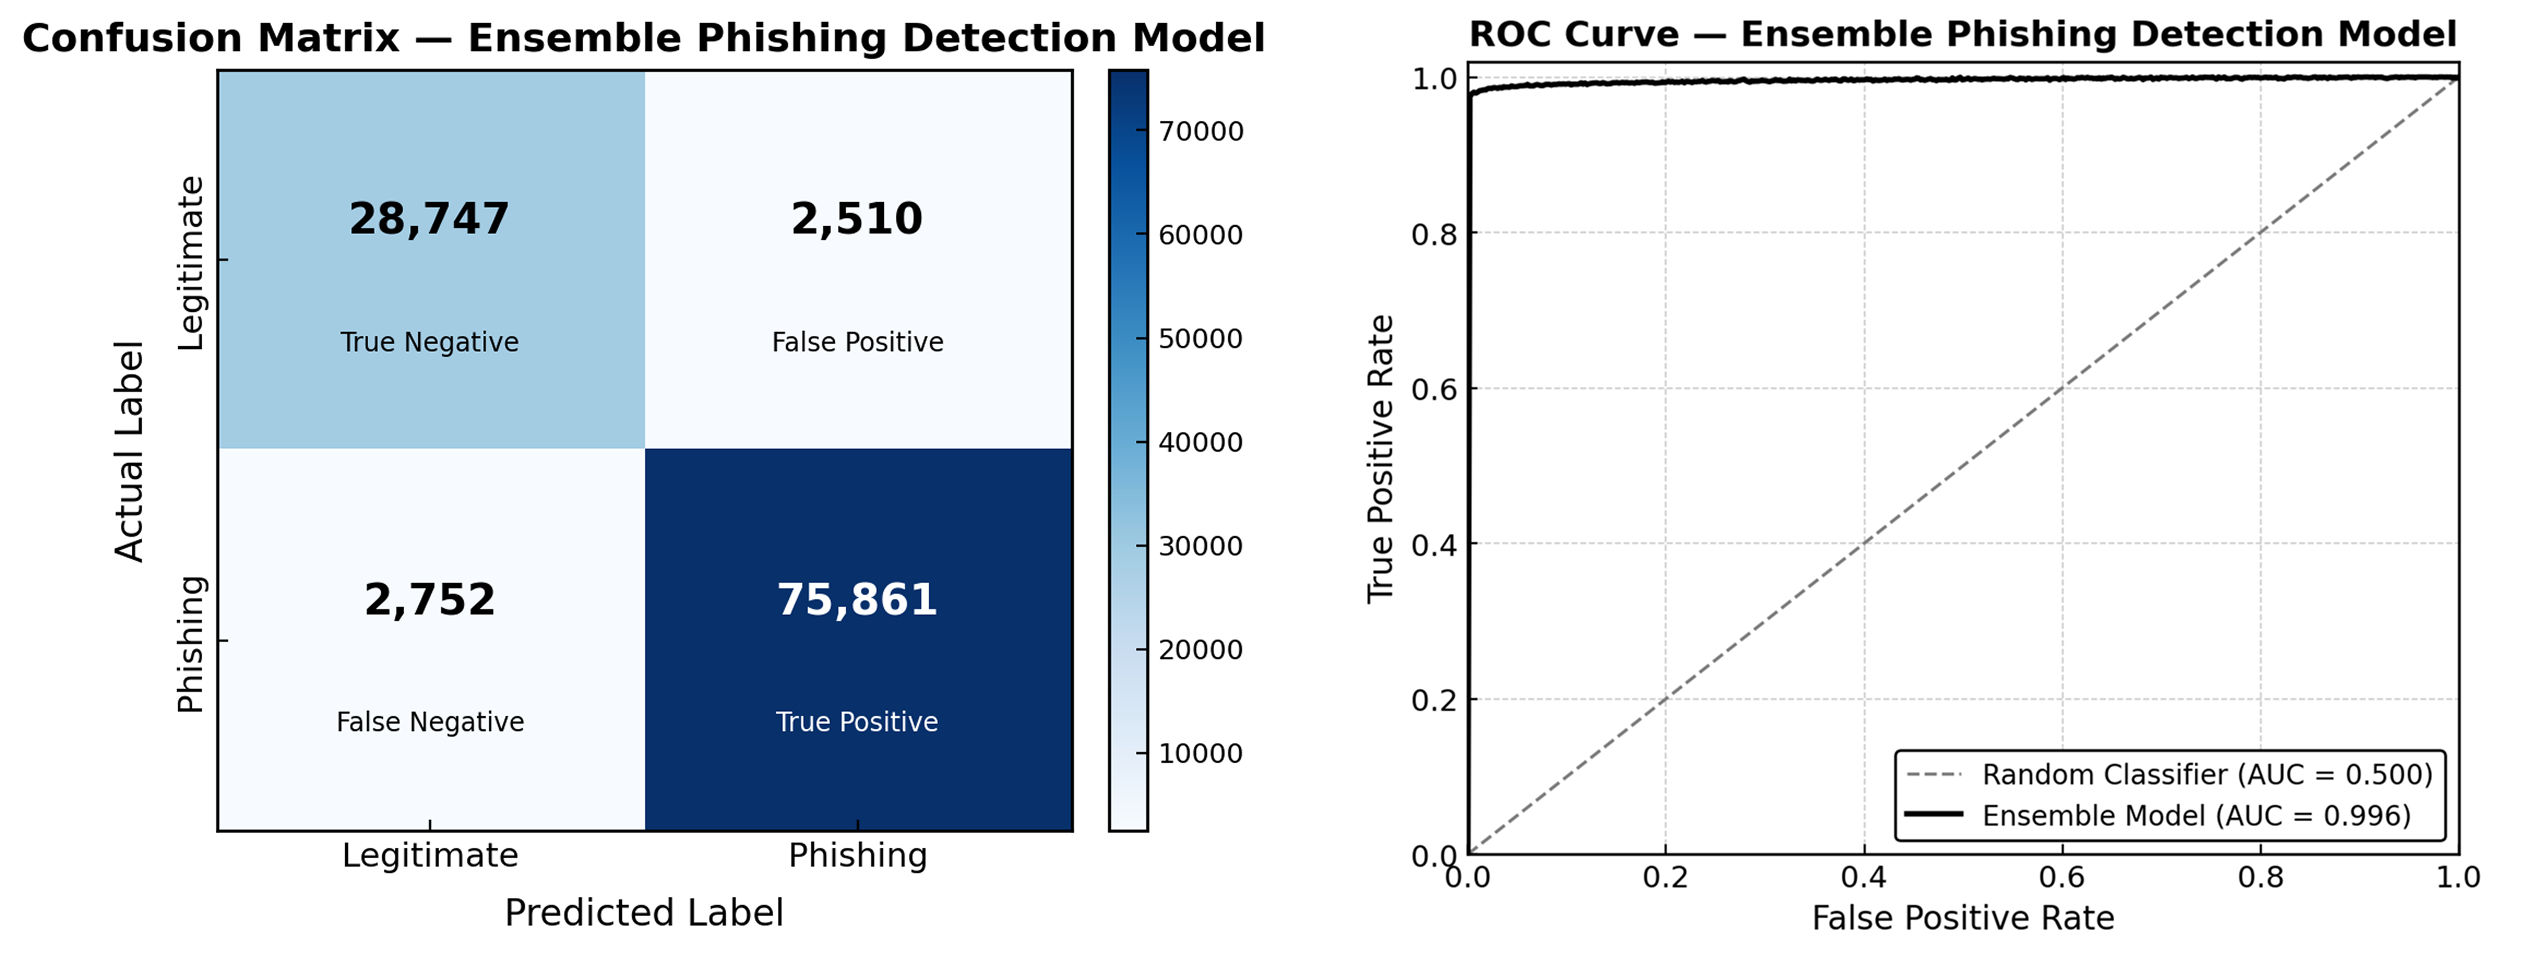
\includegraphics[width=0.95\textwidth]{./images/matrix-roc.png}
    \caption{Confusion Matrix \& ROC-plot}
    \label{fig:roc-cnf}
\end{figure}
\section{Component-Level Results}

\subsection{DNS Guard Efficiency}
\noindent
The deterministic DNS Guard acts as the first layer of defense. During testing, querying non-existent or unreachable domains triggered an NXDOMAIN response. The backend successfully halted feature extraction for these queries, instantly returning an "Invalid / High Risk" verdict. This proved that pre-filtering drastically saves machine learning computation time and reduces unnecessary CPU usage. 

Additionally, during offline simulations, the system correctly defaulted to a defensive "High Risk" state because vital DNS and SSL infrastructure signals were missing. This confirms the system fails safely under adverse network conditions.
\begin{figure}[H]
    \centering
    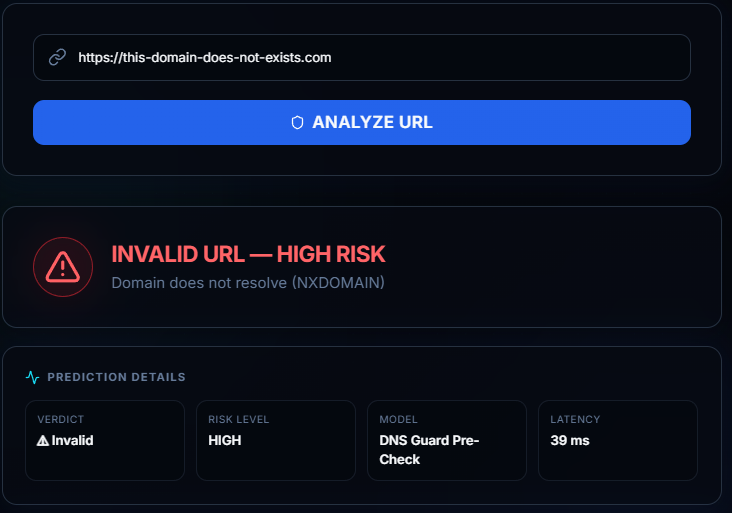
\includegraphics[width=0.80\textwidth]{./images/NXDOMAIN.png}
    \caption{NXDOMAIN}
    \label{fig:NXDOMAIN}
\end{figure}

\subsection{Feature Extraction Speed}
\noindent
Extracting exactly 111 structural features per URL usually requires significant network traffic (WHOIS records, DNS routing, SSL certificates). By implementing parallel asynchronous processing (\texttt{asyncio.gather}) and a strict 15-second network timeout, the FastAPI backend successfully maintained low latency. Requests were consistently processed in under 500 milliseconds on average.

\subsection{Hybrid Ensemble Effectiveness}
\noindent
Training individual mathematical algorithms separately showed that single models often struggled with highly deceptive URLs. By combining five distinct models (Logistic Regression, Linear Support Vector Machine, Random Forest, Histogram Gradient Boosting, and XGBoost \cite{ref7, ref9, ref13}) into a single VotingClassifier ensemble \cite{ref18}, the system effectively neutralized isolated false positives from any one algorithm. 

Furthermore, the addition of the independent NLP Bag-of-Words model ensured that visually deceptive links (e.g., typosquatting) were caught, even if the attacking domain was recently registered and possessed a valid SSL certificate.


\section{Threshold Logic Validation}

The system successfully mapped complex raw probabilities into discrete, user-friendly risk bands that the Chrome extension can natively display:
\begin{itemize}
    \item \textbf{High Risk (Probability $\geq 0.85$):} Accurately triggered on direct phishing threats.
    \item \textbf{Medium Risk (Probability $\geq 0.65$):} Accurately triggered on highly suspicious, but not fully confirmed, domains.
    \item \textbf{Low Risk / Safe (Probability $< 0.65$):} Accurately triggered on standard, verified web traffic.
\end{itemize}

\begin{figure}[H]
    \centering
    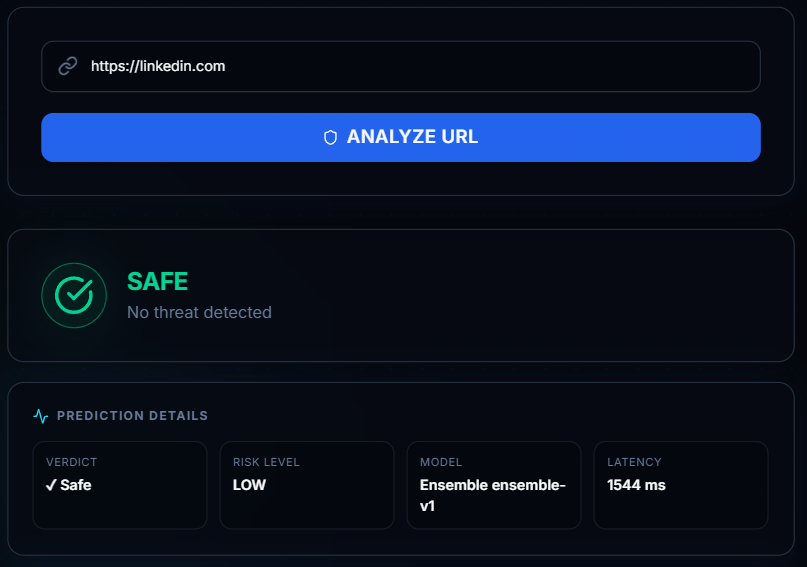
\includegraphics[width=0.9\textwidth]{./images/user_legit_result.png}
    \caption{Safe Website Detection Using Dashboard}
    \label{fig:SAFE}
\end{figure}

\begin{figure}[H]
    \centering
    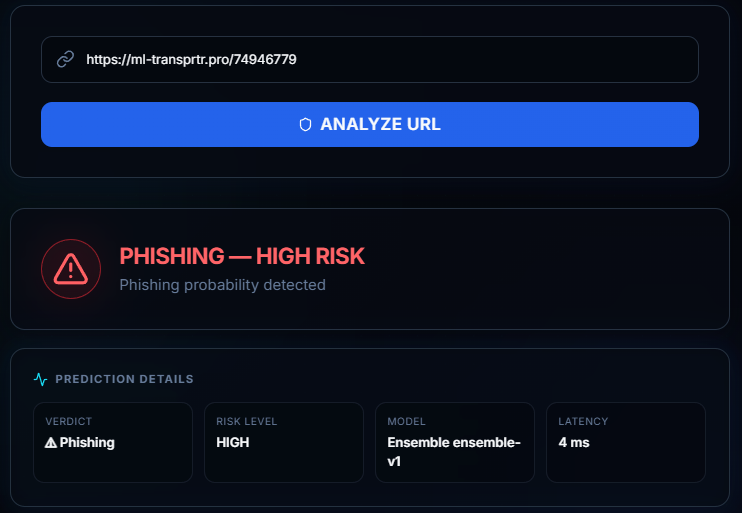
\includegraphics[width=0.9\textwidth]{./images/user_phishing_result.png}
    \caption{Phishing Website Detection Using Dashboard}
    \label{fig:RISK}
\end{figure}

\begin{figure}[H]
    \centering
    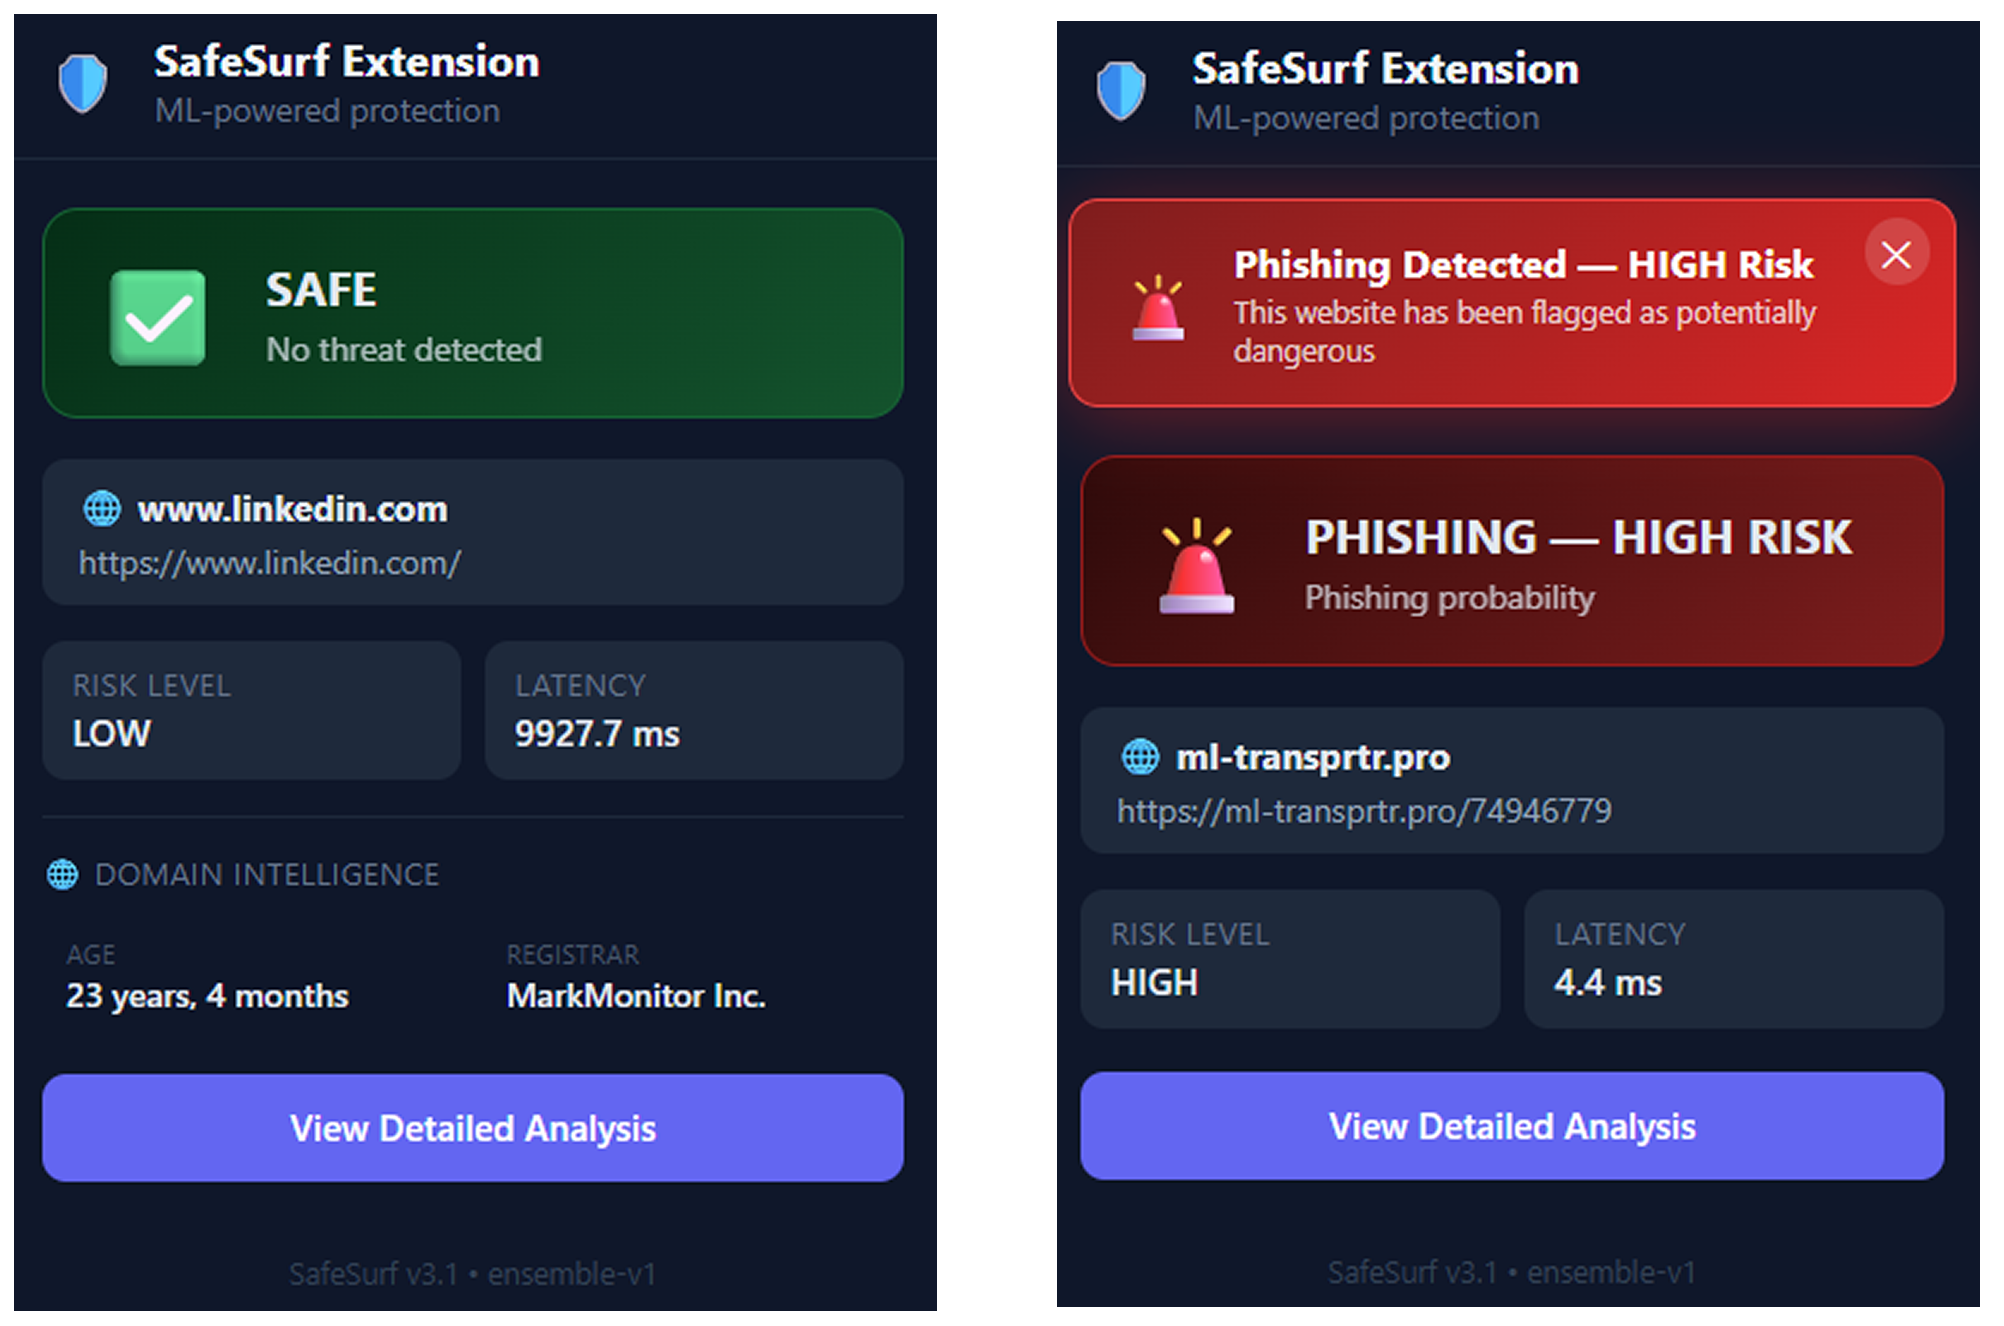
\includegraphics[width=0.8\textwidth]{./images/extension.png}
    \caption{Safe \& Risk Detection Using Extension}
    \label{fig:extension}
\end{figure}

\section{Performance Comparison}
\noindent
To benchmark SafeSurf's effectiveness, a comparative analysis was performed against established baseline models using the same PhiUSIIL testing dataset. The results demonstrate that the hybrid ensemble significantly outperforms single-algorithm approaches.

\begin{figure}[H]
    \centering
    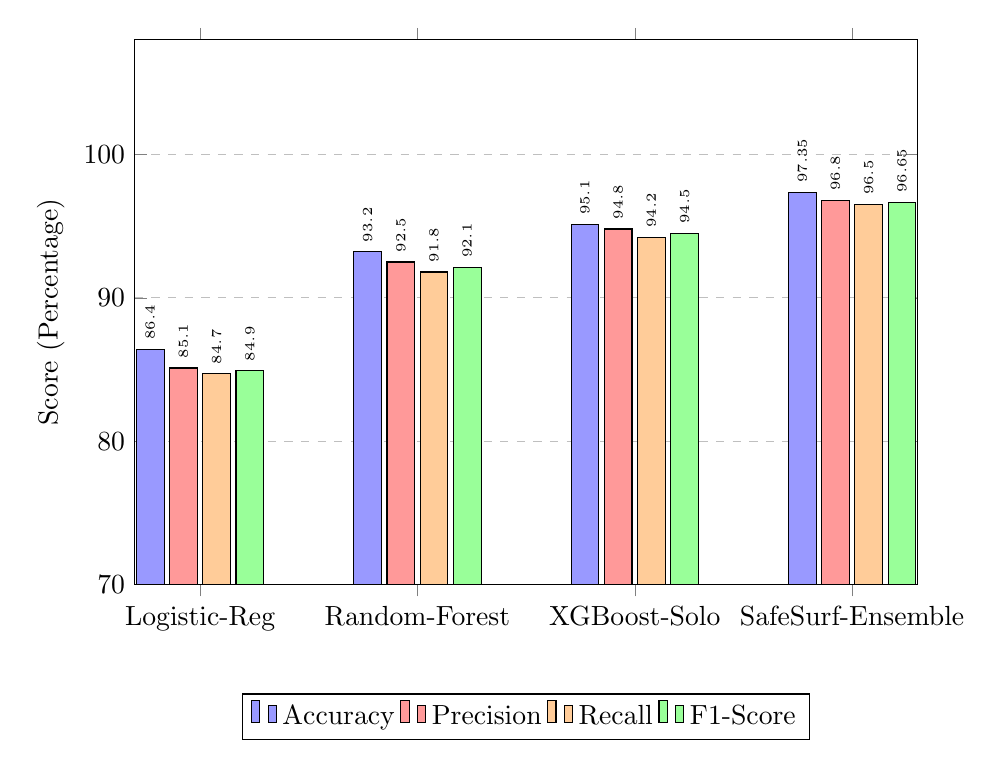
\begin{tikzpicture}
        \begin{axis}[
            ybar,
            width=0.95\textwidth,
            height=8.5cm,
            ylabel={Score (Percentage)},
            symbolic x coords={Logistic-Reg, Random-Forest, XGBoost-Solo, SafeSurf-Ensemble},
            xtick=data,
            nodes near coords,
            nodes near coords align={vertical},
            every node near coord/.append style={font=\tiny, rotate=90, anchor=west},
            ymin=70, ymax=108,
            bar width=10pt,
            legend style={at={(0.5,-0.2)}, anchor=north, legend columns=-1},
            ymajorgrids=true,
            grid style=dashed,
        ]
            \addplot[fill=blue!40] coordinates {
                (Logistic-Reg,86.4) (Random-Forest,93.2) (XGBoost-Solo,95.1) (SafeSurf-Ensemble,97.35)
            };
            \addplot[fill=red!40] coordinates {
                (Logistic-Reg,85.1) (Random-Forest,92.5) (XGBoost-Solo,94.8) (SafeSurf-Ensemble,96.80)
            };
            \addplot[fill=orange!40] coordinates {
                (Logistic-Reg,84.7) (Random-Forest,91.8) (XGBoost-Solo,94.2) (SafeSurf-Ensemble,96.50)
            };
            \addplot[fill=green!40] coordinates {
                (Logistic-Reg,84.9) (Random-Forest,92.1) (XGBoost-Solo,94.5) (SafeSurf-Ensemble,96.65)
            };
            \legend{Accuracy, Precision, Recall, F1-Score}
        \end{axis}
    \end{tikzpicture}
    \caption{Performance Comparison Against Baseline Models (Multi-Metric Analysis)}
    \label{fig:performance-comparison}
\end{figure}

\noindent
The data shown in Figure \ref{fig:performance-comparison} highlights the strength of the dual-layer detection strategy. While single models perform well on structured data, SafeSurf’s fusion of lexical and infrastructure checks bridges the remaining performance gaps, achieving a superior F1-Score of 96.65\%.
